\begin{question}[section=,name={},difficulty=,quantity=,type=thr,tags={20151210}]
	Skizzieren Sie den Modus $TE_{10}$ eines Rechteckhohlleiters mit Wellenausbreitung in z-Richtung (alle drei Schnitte)! (\addpoints{2})
	
	%\\ \textbf{Hinweis:}\\
	
\end{question}
\begin{solution}
	\begin{figure}[H]
		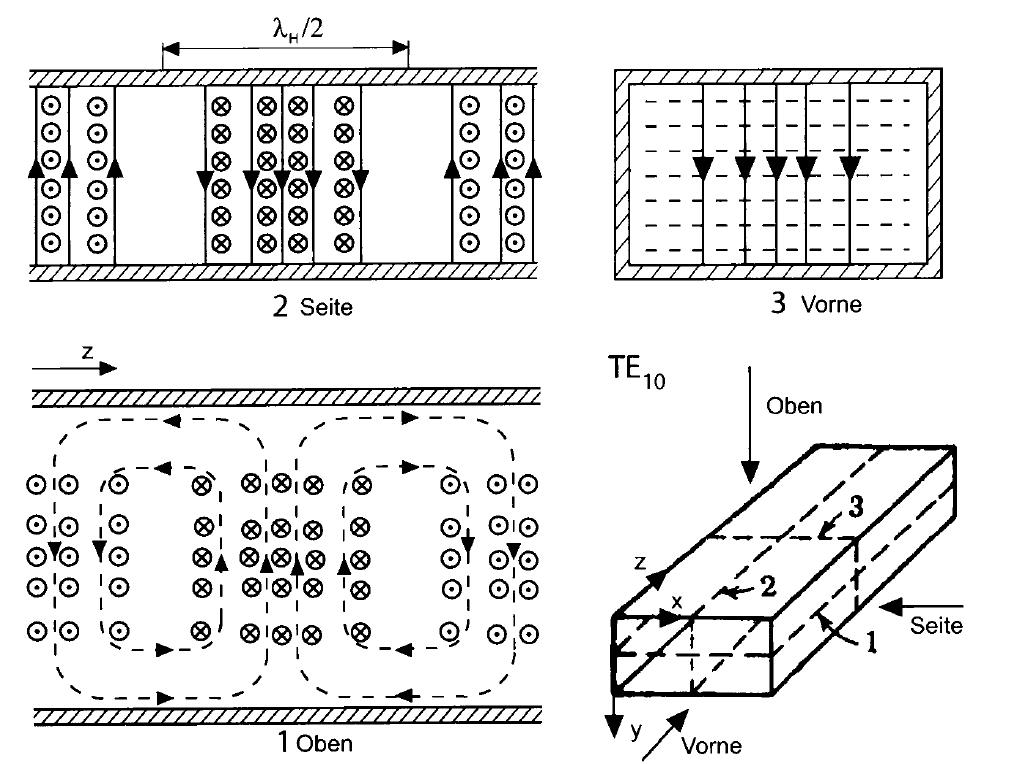
\includegraphics[width=14cm]{./opn/exm/thr/chp/6/2/bild.jpeg}
	\end{figure}
\end{solution}